\section{Convolutional Neural Networks}
\begin{frame}{\insertsec}
    This type of networks are a bit different because instead of computing the activations by
    multiplying the previous ones with the weight matrix it convolutes the previous activations 
    (denoted by $*$):
    
    \begin{align*}
        \bm{a}^{[l]} &= g(\bm{W}^{[l]}\cdot \bm{a}^{[l - 1]} + \bm{b}^{[l]}) \\
        \text{Becomes:} \\
        \bm{a}^{[l]} &= g(\bm{W}^{[l]} * \bm{a}^{[l-1]} + \bm{b}^{[l]})
    \end{align*}
\end{frame}

\subsection{Convolution Operation}
\begin{frame}{\insertsubsec}
    \begin{alertblock}{Important}
        What we call \textit{Convolution} in ML it's actually the \textit{Cross-Correlation} operation
        in signal analysis.
    \end{alertblock}
    
    \begin{align*}
        \left(
        \begin{array}{cccccc}
            10 & \cellcolor{green!20}10 & \cellcolor{green!20}10 & \cellcolor{green!20}0 & 0 & 0 \\
            10 & \cellcolor{green!20}10 & \cellcolor{green!20}10 & \cellcolor{green!20}0 & 0 & 0 \\
            10 & \cellcolor{green!20}10 & \cellcolor{green!20}10 & \cellcolor{green!20}0 & 0 & 0 \\
            10 & 10 & 10 & 0 & 0 & 0 \\
            10 & 10 & 10 & 0 & 0 & 0 \\
            10 & 10 & 10 & 0 & 0 & 0 \\
        \end{array}
        \right)
        *
        \left(
        \begin{array}{ccc}
            1 & 0 & -1 \\
            1 & 0 & -1 \\ 
            1 & 0 & -1 \\
        \end{array}
        \right)
        = 
        \left(
        \begin{array}{cccc}
            0 & \cellcolor{green!20}30 & 30 & 0 \\
            0 & 30 & 30 & 0 \\
            0 & 30 & 30 & 0 \\
            0 & 30 & 30 & 0 \\
        \end{array}
        \right)
    \end{align*}
    $$
        10 \cdot 1 + 10 \cdot 1 + 10 \cdot 1 +
        10 \cdot 0 + 10 \cdot 0 + 10 \cdot 0 +
        0 \cdot -1 + 0 \cdot -1 + 0 \cdot -1 = 30
    $$
\end{frame}

\begin{frame}
    With convolutions the Neural Network parameters ($w$) are the convolution matrix elements
    and so we do multiple convolutions to filter different features.
    

\begin{figure}[H]
    \tikzset{pics/3DBox/.style n args={3}{code={
        \tikzstyle{box}=[blue, fill=blue!20];
        \draw[box] (0, 0, 0) -- (0, #2, 0) -- (#1, #2, 0) -- (#1, 0, 0) -- cycle;
        \draw[box] (#1, 0, 0) -- (#1, 0, -#3) -- (#1, #2, -#3) -- (#1, #2, 0) -- cycle;
        \draw[box] (0, #2, 0) -- (#1, #2, 0) -- (#1, #2, -#3) -- (0, #2, -#3) -- cycle; 
    }}}

    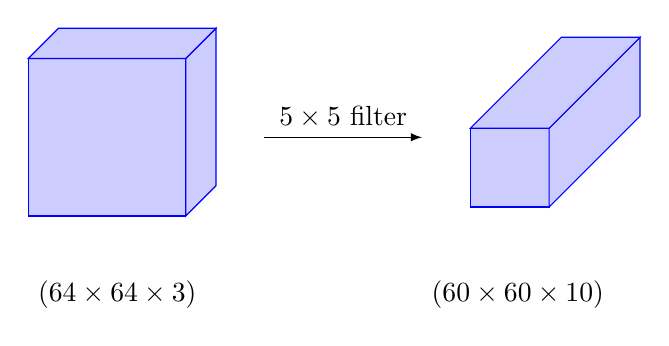
\begin{tikzpicture}
        \path pic at (0, 0, 0) {3DBox={2}{2}{1}};
        \path pic at (6, .5, 1) {3DBox={1}{1}{3}};
        \draw [-latex] (3, 1, 0) -- (5, 1, 0) node[above, midway] {$5 \times 5$ filter};

        \node [anchor=west] at (0, -1, 0) {$(64 \times 64 \times 3)$};
        \node [anchor=west] at (5 , -1, 0) {$(60 \times 60 \times 10)$};
    \end{tikzpicture}
\end{figure}


\end{frame}

\subsection{Pooling operation}
\begin{frame}{\insertsubsec}
    We use pooling to reduce the volume width and height size
    \begin{block}{Max-Pooling}
        \begin{align*}
            \operatorname{max\,pool}
            \left(
            \begin{array}{cccc}
                \cellcolor{green!20} 0 & \cellcolor{green!20} 7 & 12 &  9 \\
                \cellcolor{green!20}15 & \cellcolor{green!20} 3 & 22 &  6 \\
                 2 & 12 &  8 &  3 \\
                 6 &  2 & 18 &  3 \\
            \end{array}
            \right)
            =
            \left(
            \begin{array}{cc}
                \cellcolor{green!20}15 & 22 \\
                12 & 18
            \end{array}
            \right)
        \end{align*}
    \end{block}

    \begin{block}{Avg-Pooling}
        \begin{align*}
            \operatorname{avg\,pool}
            \left(
            \begin{array}{cccc}
                \cellcolor{green!20} 0 & \cellcolor{green!20} 7 & 12 &  9 \\
                \cellcolor{green!20}15 & \cellcolor{green!20} 3 & 22 &  6 \\
                 2 & 12 &  8 &  3 \\
                 6 &  2 & 18 &  3 \\
            \end{array}
            \right)
            =
            \left(
            \begin{array}{cc}
                \cellcolor{green!20}6.25 & 12.25 \\
                5.50 & 8.00
            \end{array}
            \right)
        \end{align*}
    \end{block}
\end{frame}

\subsection{Residual Networks}
\begin{frame}{\insertsubsec}
    They are a type of network that can learn the identity function thus allowing us to do
    very deep networks.
    \def\layersep{1.5cm}

\begin{figure}[H]
    \begin{tikzpicture}[node distance=\layersep]
        \tikzstyle{block}=[rectangle, fill=green!30, inner sep = 5pt]
        \node[block] (R0) at (0, 0) {Block 0};
        \node[left = .75 of R0] (A0) {};
        \node[above = .75 of R0] (A1) {};
        \node[block, left = .75 of A0, text width = 2cm] (I0) {Previous blocks};
        \node[block, right = of R0] (R1) {Block 1};
        \node[right = 1 of R1] (A2) {};

        % Arrows
        \draw [-latex] (I0) -- (R0) node[above, near start] {$a^{[l]}$};
        \draw [-latex] (R0) -- (R1) node[above, midway] {$a^{[l + 1]}$};
        \draw (A0.center) |- (A1.center); 
        \draw [-latex] (A1.center) -| (R1.north);
        \draw [-latex] (R1) -- (A2) node[above, midway] {$a^{[l + 2]}$};
    \end{tikzpicture}
\end{figure}

    \begin{align*}
        \bm{a}^{[l+2]} = 
        g(\underbrace{W^{[l+2]} \cdot \bm{a}^{[l + 1]} + \bm{b}^{[l + 2]}}
        _{0 \text{ if using regularization}} + \bm{a}^{[l]})
    \end{align*}
\end{frame}